\section{Introduction}
\begin{frame}
	\frametitle{Kilobots}
	\begin{columns}		
		\begin{column}{0.5\textwidth}
			\textbf{Specifications}
			\vspace{0.2cm}
			\begin{itemize}
				\item ATmega 328p processor 
				\item Li-Ion 3.7V battery 
				\item One IR transmitter-receiver pair 
				\item One light sensor 
				\item Two vibration motors (1 cm/sec, 45 degrees/sec)
			\end{itemize}
		\end{column}
	\begin{column}{0.5\textwidth}
		\begin{figure}
			\centering
			\fbox{\includegraphics[scale=0.03]{images/kilobot.jpg}}
			\vspace{0.2cm}
			\caption{Kilobot}
		\end{figure}
	\end{column}
	\end{columns}
\end{frame}

\begin{frame}
	\frametitle{About Kilobots \cite{kilobotics_manual}}
	\begin{columns}
		\begin{column}{0.5\textwidth}
			\begin{figure}
				\centering
				\fbox{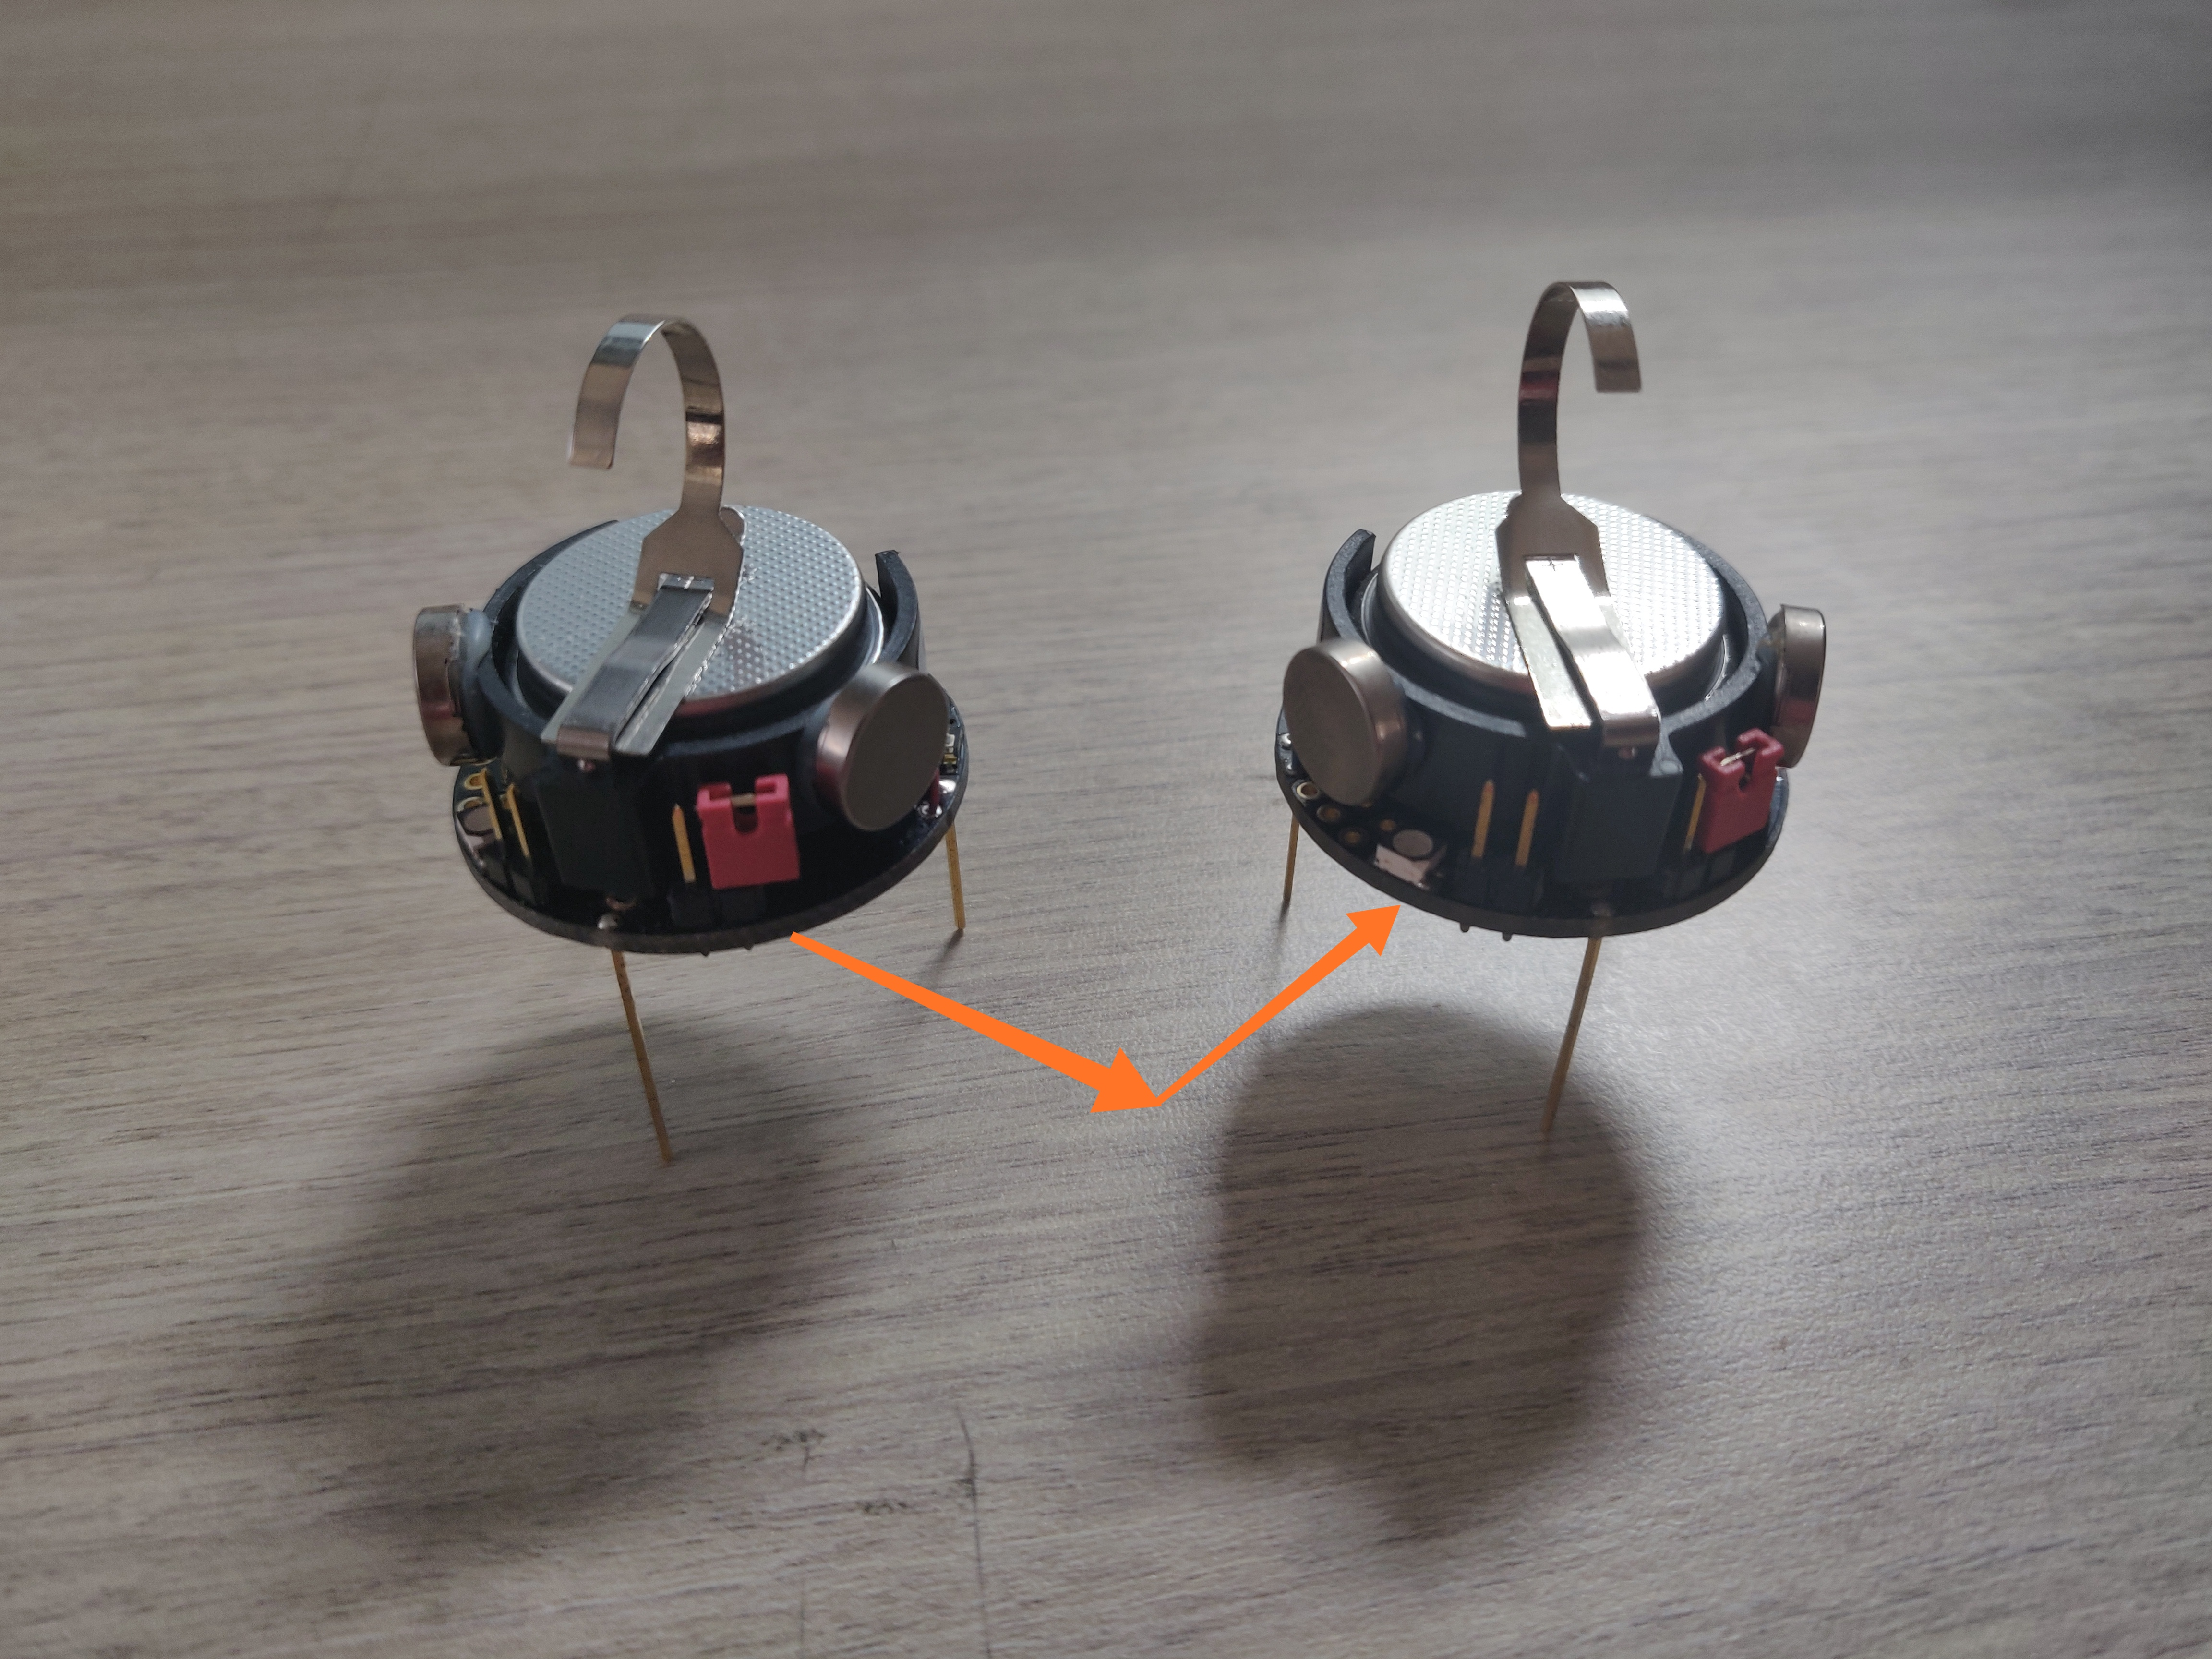
\includegraphics[scale=0.03]{images/IR-communication.jpg}}
				\vspace{0.2cm}
				\caption{Communication between two Kilobots}
			\end{figure}
		\end{column}
		\begin{column}{0.5\textwidth}
			\begin{itemize}
				\item Reflecting IR light
				\item Communication up to 7 cm (32kb/s) away 
				\item Using over-head controller(OHC)
			\end{itemize}
		\end{column}
	\end{columns}
\end{frame}

\begin{frame}
	\frametitle{KiloGUI}
	\begin{itemize}
		\item Upload new programs 
		\item Motor calibration of the robots    
		\item Set unique ID manually
	\end{itemize}
\end{frame}

\begin{frame}
	\frametitle{KiloGUI}
	\begin{columns}[b]
	\begin{column}{0.5\textwidth}
		\begin{figure}
			\centering
			\includegraphics[scale=0.35]{images/kilogui.png}
			\vspace{0.2cm}
			\caption{KiloGUI}
		\end{figure}
	\end{column}
	\begin{column}{0.5\textwidth}	
		\begin{figure}
			\includegraphics[scale=0.35]{images/kilogui-motor-calib.png}
			\vspace{0.2cm}
			\caption{Motor Calibration}
		\end{figure}
	\end{column}
\end{columns}
\end{frame}

\begin{frame}{Abstract}
\begin{itemize}
    \item Algorithm for self-assembly in Kilobots.
    \item According to \cite{MR-AC-RN:2014}, self-assembly algorithm composes three primitive collective behaviors 
    \begin{itemize}
        \item Edge-following
        \item Gradient Formation
        \item Localization 
    \end{itemize}
    
\end{itemize}
\end{frame}

\begin{frame}{Previous and Present work}
\textbf{Previous work}
\begin{itemize}
    \item Localization
\end{itemize}
\textbf{Present work}
\begin{itemize}
    \item Gradient formation
    \item Edge-following
\end{itemize}

\end{frame}

